\documentclass[tikz,border=0mm]{standalone}
\usepackage[utf8]{inputenc}
\usepackage{unicode-math}
\usepackage{amsmath}
\usepackage{siunitx}
\usepackage{mhchem}
\usepackage{tikz}


\begin{document}
\definecolor{backgroundColor}{rgb}{1.0, 1.0, 1.0}

\pagecolor{backgroundColor}


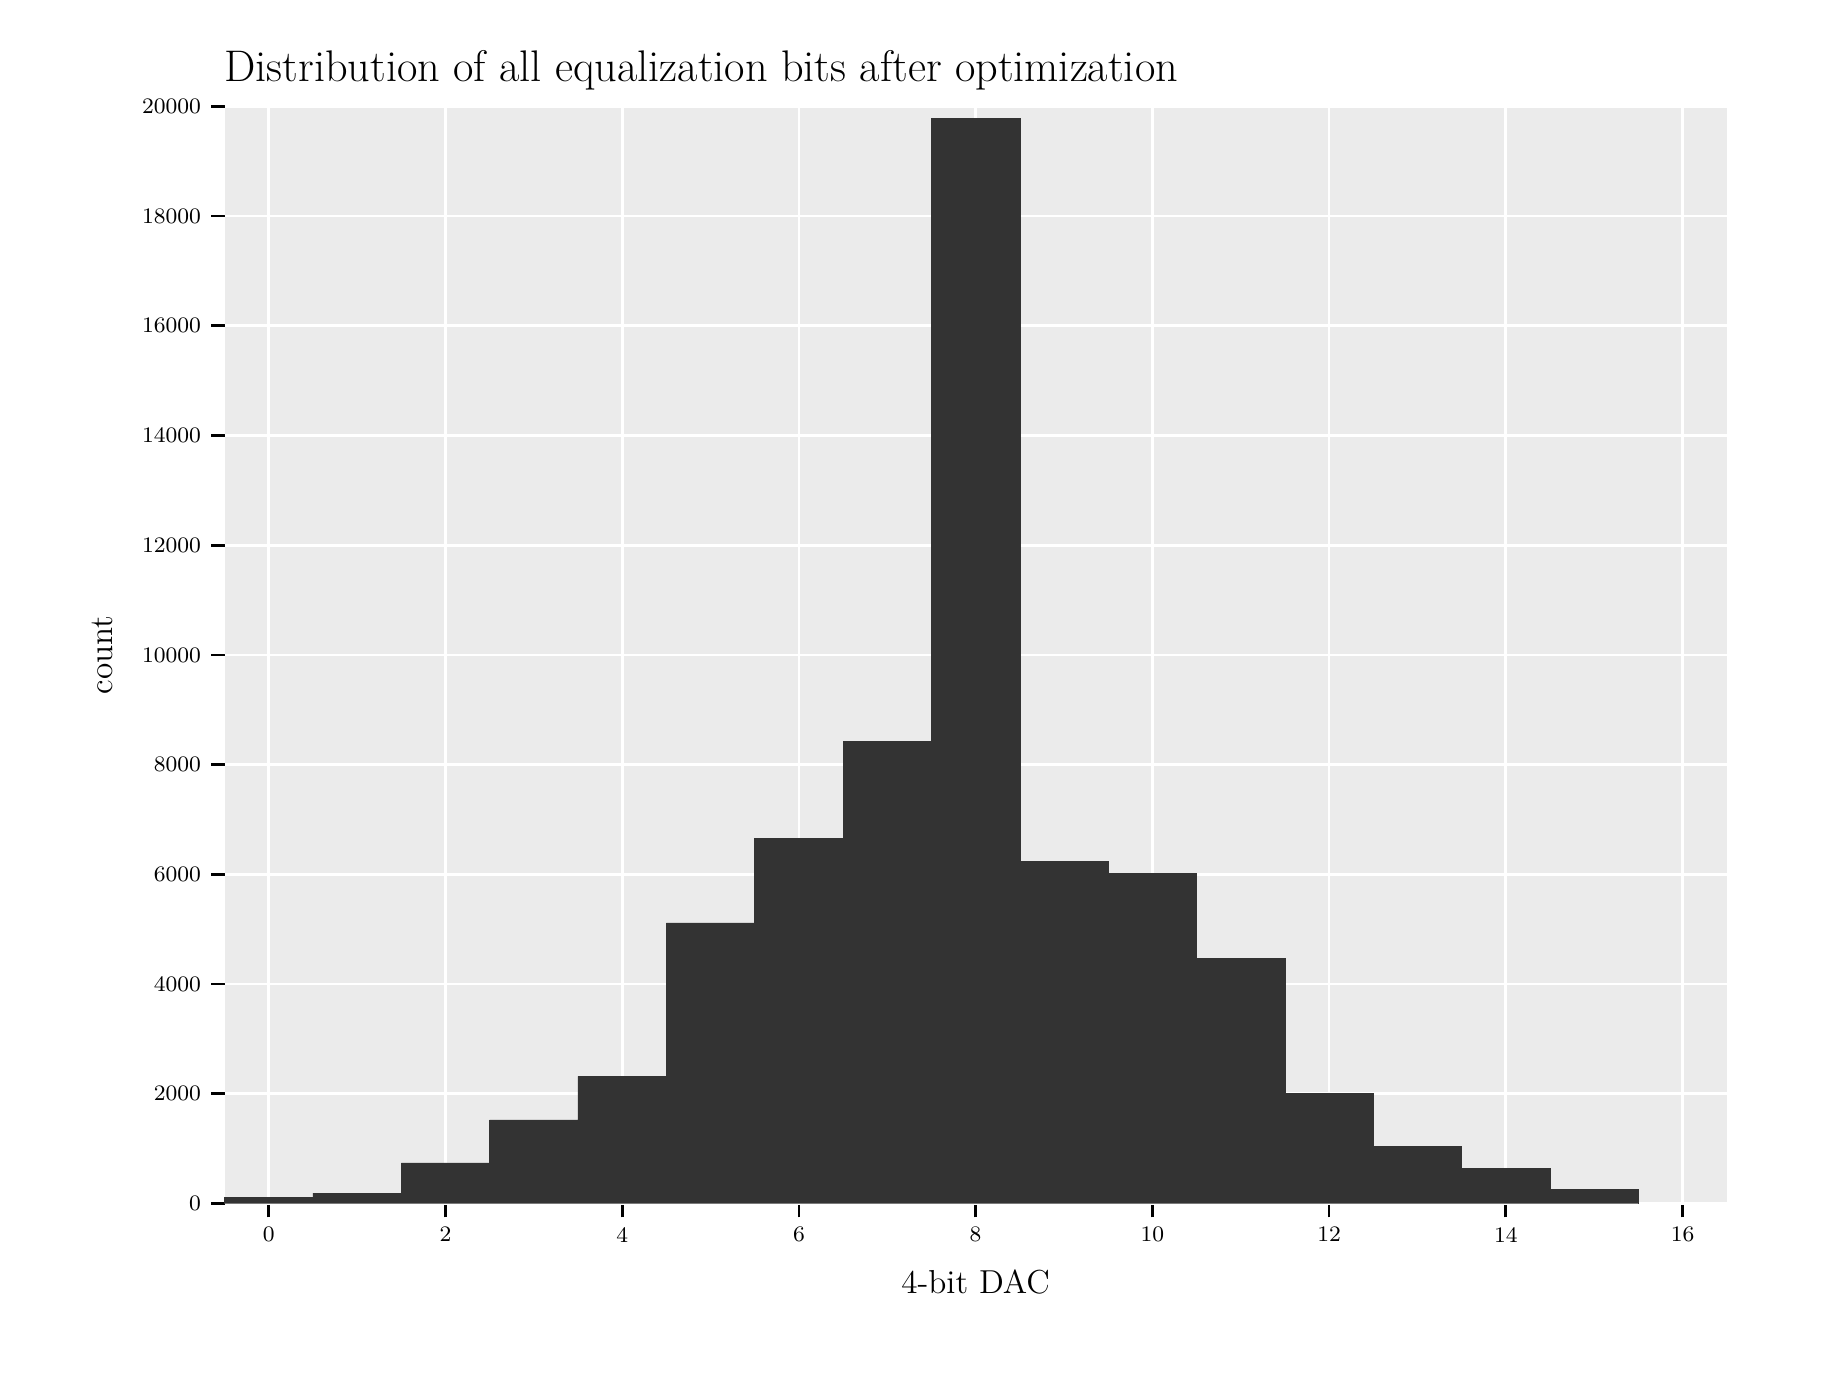
\begin{tikzpicture}[every node/.style={outer sep=0pt, inner sep=0pt}]
\path[use as bounding box] (0, 0) rectangle (640.0bp, 480.0bp) ;
\definecolor{drawColor}{rgb}{0.0, 0.0, 0.0}
\definecolor{fillColor}{rgb}{1.0, 1.0, 1.0}

\draw [color = drawColor, fill = fillColor, draw opacity = 0.0, fill opacity = 1.0, line width = 0.0bp] (0.0000bp, 480.0000bp) rectangle (640.0000bp, 0.0000bp) ;
\node [right, font=\fontsize{16.0}{19.2}\selectfont
, anchor=west] at (70.8661bp, 464.5722bp){Distribution of all equalization bits after optimization} ;
\definecolor{drawColor}{rgb}{0.0, 0.0, 0.0}
\definecolor{fillColor}{rgb}{0.9200000166893005, 0.9200000166893005, 0.9200000166893005}

\draw [color = drawColor, fill = fillColor, draw opacity = 0.0, fill opacity = 1.0, line width = 0.0bp] (70.8661bp, 451.6535bp) rectangle (611.6535bp, 56.6929bp) ;
\definecolor{drawColor}{rgb}{0.0, 0.0, 0.0}
\definecolor{fillColor}{rgb}{0.0, 0.0, 0.0}

\draw [color = drawColor, fill = fillColor, draw opacity = 1.0, fill opacity = 0.0, line width = 1.0bp] (86.7717bp, 51.6929bp)--(86.7717bp, 56.6929bp) ;
\draw [color = drawColor, fill = fillColor, draw opacity = 1.0, fill opacity = 0.0, line width = 1.0bp] (150.3937bp, 51.6929bp)--(150.3937bp, 56.6929bp) ;
\draw [color = drawColor, fill = fillColor, draw opacity = 1.0, fill opacity = 0.0, line width = 1.0bp] (214.0157bp, 51.6929bp)--(214.0157bp, 56.6929bp) ;
\draw [color = drawColor, fill = fillColor, draw opacity = 1.0, fill opacity = 0.0, line width = 1.0bp] (277.6378bp, 51.6929bp)--(277.6378bp, 56.6929bp) ;
\draw [color = drawColor, fill = fillColor, draw opacity = 1.0, fill opacity = 0.0, line width = 1.0bp] (341.2598bp, 51.6929bp)--(341.2598bp, 56.6929bp) ;
\draw [color = drawColor, fill = fillColor, draw opacity = 1.0, fill opacity = 0.0, line width = 1.0bp] (404.8819bp, 51.6929bp)--(404.8819bp, 56.6929bp) ;
\draw [color = drawColor, fill = fillColor, draw opacity = 1.0, fill opacity = 0.0, line width = 1.0bp] (468.5039bp, 51.6929bp)--(468.5039bp, 56.6929bp) ;
\draw [color = drawColor, fill = fillColor, draw opacity = 1.0, fill opacity = 0.0, line width = 1.0bp] (532.1260bp, 51.6929bp)--(532.1260bp, 56.6929bp) ;
\draw [color = drawColor, fill = fillColor, draw opacity = 1.0, fill opacity = 0.0, line width = 1.0bp] (595.7480bp, 51.6929bp)--(595.7480bp, 56.6929bp) ;
\node [font=\fontsize{8.0}{9.6}\selectfont
] at (86.7717bp, 45.4590bp){0} ;
\node [font=\fontsize{8.0}{9.6}\selectfont
] at (150.3937bp, 45.5433bp){2} ;
\node [font=\fontsize{8.0}{9.6}\selectfont
] at (214.0157bp, 45.5031bp){4} ;
\node [font=\fontsize{8.0}{9.6}\selectfont
] at (277.6378bp, 45.4590bp){6} ;
\node [font=\fontsize{8.0}{9.6}\selectfont
] at (341.2598bp, 45.4590bp){8} ;
\node [font=\fontsize{8.0}{9.6}\selectfont
] at (404.8819bp, 45.4590bp){10} ;
\node [font=\fontsize{8.0}{9.6}\selectfont
] at (468.5039bp, 45.5433bp){12} ;
\node [font=\fontsize{8.0}{9.6}\selectfont
] at (532.1260bp, 45.5031bp){14} ;
\node [font=\fontsize{8.0}{9.6}\selectfont
] at (595.7480bp, 45.4590bp){16} ;
\draw [color = drawColor, fill = fillColor, draw opacity = 1.0, fill opacity = 0.0, line width = 1.0bp] (70.8661bp, 56.6929bp)--(65.8661bp, 56.6929bp) ;
\draw [color = drawColor, fill = fillColor, draw opacity = 1.0, fill opacity = 0.0, line width = 1.0bp] (70.8661bp, 96.1890bp)--(65.8661bp, 96.1890bp) ;
\draw [color = drawColor, fill = fillColor, draw opacity = 1.0, fill opacity = 0.0, line width = 1.0bp] (70.8661bp, 135.6850bp)--(65.8661bp, 135.6850bp) ;
\draw [color = drawColor, fill = fillColor, draw opacity = 1.0, fill opacity = 0.0, line width = 1.0bp] (70.8661bp, 175.1811bp)--(65.8661bp, 175.1811bp) ;
\draw [color = drawColor, fill = fillColor, draw opacity = 1.0, fill opacity = 0.0, line width = 1.0bp] (70.8661bp, 214.6772bp)--(65.8661bp, 214.6772bp) ;
\draw [color = drawColor, fill = fillColor, draw opacity = 1.0, fill opacity = 0.0, line width = 1.0bp] (70.8661bp, 254.1732bp)--(65.8661bp, 254.1732bp) ;
\draw [color = drawColor, fill = fillColor, draw opacity = 1.0, fill opacity = 0.0, line width = 1.0bp] (70.8661bp, 293.6693bp)--(65.8661bp, 293.6693bp) ;
\draw [color = drawColor, fill = fillColor, draw opacity = 1.0, fill opacity = 0.0, line width = 1.0bp] (70.8661bp, 333.1654bp)--(65.8661bp, 333.1654bp) ;
\draw [color = drawColor, fill = fillColor, draw opacity = 1.0, fill opacity = 0.0, line width = 1.0bp] (70.8661bp, 372.6614bp)--(65.8661bp, 372.6614bp) ;
\draw [color = drawColor, fill = fillColor, draw opacity = 1.0, fill opacity = 0.0, line width = 1.0bp] (70.8661bp, 412.1575bp)--(65.8661bp, 412.1575bp) ;
\draw [color = drawColor, fill = fillColor, draw opacity = 1.0, fill opacity = 0.0, line width = 1.0bp] (70.8661bp, 451.6535bp)--(65.8661bp, 451.6535bp) ;
\node [left, font=\fontsize{8.0}{9.6}\selectfont
, anchor=east] at (62.3865bp, 56.6929bp){0} ;
\node [left, font=\fontsize{8.0}{9.6}\selectfont
, anchor=east] at (62.3865bp, 96.1890bp){2000} ;
\node [left, font=\fontsize{8.0}{9.6}\selectfont
, anchor=east] at (62.3865bp, 135.6850bp){4000} ;
\node [left, font=\fontsize{8.0}{9.6}\selectfont
, anchor=east] at (62.3865bp, 175.1811bp){6000} ;
\node [left, font=\fontsize{8.0}{9.6}\selectfont
, anchor=east] at (62.3865bp, 214.6772bp){8000} ;
\node [left, font=\fontsize{8.0}{9.6}\selectfont
, anchor=east] at (62.3865bp, 254.1732bp){10000} ;
\node [left, font=\fontsize{8.0}{9.6}\selectfont
, anchor=east] at (62.3865bp, 293.6693bp){12000} ;
\node [left, font=\fontsize{8.0}{9.6}\selectfont
, anchor=east] at (62.3865bp, 333.1654bp){14000} ;
\node [left, font=\fontsize{8.0}{9.6}\selectfont
, anchor=east] at (62.3865bp, 372.6614bp){16000} ;
\node [left, font=\fontsize{8.0}{9.6}\selectfont
, anchor=east] at (62.3865bp, 412.1575bp){18000} ;
\node [left, font=\fontsize{8.0}{9.6}\selectfont
, anchor=east] at (62.3865bp, 451.6535bp){20000} ;
\node [font=\fontsize{12.0}{14.4}\selectfont
] at (341.2598bp, 28.3465bp){4-bit DAC} ;
\node [rotate = 90.0, font=\fontsize{12.0}{14.4}\selectfont
] at (26.8693bp, 254.1732bp){count} ;
\definecolor{drawColor}{rgb}{1.0, 1.0, 1.0}
\definecolor{fillColor}{rgb}{0.0, 0.0, 0.0}

\draw [color = drawColor, fill = fillColor, draw opacity = 1.0, fill opacity = 0.0, line width = 1.0bp] (86.7717bp, 451.6535bp)--(86.7717bp, 56.6929bp) ;
\draw [color = drawColor, fill = fillColor, draw opacity = 1.0, fill opacity = 0.0, line width = 1.0bp] (150.3937bp, 451.6535bp)--(150.3937bp, 56.6929bp) ;
\draw [color = drawColor, fill = fillColor, draw opacity = 1.0, fill opacity = 0.0, line width = 1.0bp] (214.0157bp, 451.6535bp)--(214.0157bp, 56.6929bp) ;
\draw [color = drawColor, fill = fillColor, draw opacity = 1.0, fill opacity = 0.0, line width = 1.0bp] (277.6378bp, 451.6535bp)--(277.6378bp, 56.6929bp) ;
\draw [color = drawColor, fill = fillColor, draw opacity = 1.0, fill opacity = 0.0, line width = 1.0bp] (341.2598bp, 451.6535bp)--(341.2598bp, 56.6929bp) ;
\draw [color = drawColor, fill = fillColor, draw opacity = 1.0, fill opacity = 0.0, line width = 1.0bp] (404.8819bp, 451.6535bp)--(404.8819bp, 56.6929bp) ;
\draw [color = drawColor, fill = fillColor, draw opacity = 1.0, fill opacity = 0.0, line width = 1.0bp] (468.5039bp, 451.6535bp)--(468.5039bp, 56.6929bp) ;
\draw [color = drawColor, fill = fillColor, draw opacity = 1.0, fill opacity = 0.0, line width = 1.0bp] (532.1260bp, 451.6535bp)--(532.1260bp, 56.6929bp) ;
\draw [color = drawColor, fill = fillColor, draw opacity = 1.0, fill opacity = 0.0, line width = 1.0bp] (595.7480bp, 451.6535bp)--(595.7480bp, 56.6929bp) ;
\draw [color = drawColor, fill = fillColor, draw opacity = 1.0, fill opacity = 0.0, line width = 1.0bp] (70.8661bp, 56.6929bp)--(611.6535bp, 56.6929bp) ;
\draw [color = drawColor, fill = fillColor, draw opacity = 1.0, fill opacity = 0.0, line width = 1.0bp] (70.8661bp, 96.1890bp)--(611.6535bp, 96.1890bp) ;
\draw [color = drawColor, fill = fillColor, draw opacity = 1.0, fill opacity = 0.0, line width = 1.0bp] (70.8661bp, 135.6850bp)--(611.6535bp, 135.6850bp) ;
\draw [color = drawColor, fill = fillColor, draw opacity = 1.0, fill opacity = 0.0, line width = 1.0bp] (70.8661bp, 175.1811bp)--(611.6535bp, 175.1811bp) ;
\draw [color = drawColor, fill = fillColor, draw opacity = 1.0, fill opacity = 0.0, line width = 1.0bp] (70.8661bp, 214.6772bp)--(611.6535bp, 214.6772bp) ;
\draw [color = drawColor, fill = fillColor, draw opacity = 1.0, fill opacity = 0.0, line width = 1.0bp] (70.8661bp, 254.1732bp)--(611.6535bp, 254.1732bp) ;
\draw [color = drawColor, fill = fillColor, draw opacity = 1.0, fill opacity = 0.0, line width = 1.0bp] (70.8661bp, 293.6693bp)--(611.6535bp, 293.6693bp) ;
\draw [color = drawColor, fill = fillColor, draw opacity = 1.0, fill opacity = 0.0, line width = 1.0bp] (70.8661bp, 333.1654bp)--(611.6535bp, 333.1654bp) ;
\draw [color = drawColor, fill = fillColor, draw opacity = 1.0, fill opacity = 0.0, line width = 1.0bp] (70.8661bp, 372.6614bp)--(611.6535bp, 372.6614bp) ;
\draw [color = drawColor, fill = fillColor, draw opacity = 1.0, fill opacity = 0.0, line width = 1.0bp] (70.8661bp, 412.1575bp)--(611.6535bp, 412.1575bp) ;
\draw [color = drawColor, fill = fillColor, draw opacity = 1.0, fill opacity = 0.0, line width = 1.0bp] (70.8661bp, 451.6535bp)--(611.6535bp, 451.6535bp) ;
\definecolor{drawColor}{rgb}{0.2000000029802322, 0.2000000029802322, 0.2000000029802322}
\definecolor{fillColor}{rgb}{0.2000000029802322, 0.2000000029802322, 0.2000000029802322}

\draw [color = drawColor, fill = fillColor, draw opacity = 1.0, fill opacity = 1.0, line width = 0.2bp]
(70.8661bp, 56.6929bp)  -- 
(70.8661bp, 56.6929bp)  -- 
(70.8661bp, 59.0034bp)  -- 
(102.6772bp, 59.0034bp)  -- 
(102.6772bp, 60.4253bp)  -- 
(134.4882bp, 60.4253bp)  -- 
(134.4882bp, 71.3065bp)  -- 
(166.2992bp, 71.3065bp)  -- 
(166.2992bp, 86.7692bp)  -- 
(198.1102bp, 86.7692bp)  -- 
(198.1102bp, 102.4689bp)  -- 
(229.9213bp, 102.4689bp)  -- 
(229.9213bp, 157.7238bp)  -- 
(261.7323bp, 157.7238bp)  -- 
(261.7323bp, 188.0173bp)  -- 
(293.5433bp, 188.0173bp)  -- 
(293.5433bp, 223.1096bp)  -- 
(325.3543bp, 223.1096bp)  -- 
(325.3543bp, 447.4077bp)  -- 
(357.1654bp, 447.4077bp)  -- 
(357.1654bp, 179.7231bp)  -- 
(388.9764bp, 179.7231bp)  -- 
(388.9764bp, 175.4576bp)  -- 
(420.7874bp, 175.4576bp)  -- 
(420.7874bp, 145.0654bp)  -- 
(452.5984bp, 145.0654bp)  -- 
(452.5984bp, 96.3470bp)  -- 
(484.4094bp, 96.3470bp)  -- 
(484.4094bp, 77.2704bp)  -- 
(516.2205bp, 77.2704bp)  -- 
(516.2205bp, 69.3119bp)  -- 
(548.0315bp, 69.3119bp)  -- 
(548.0315bp, 61.8866bp)  -- 
(579.8425bp, 61.8866bp)  -- 
(579.8425bp, 56.6929bp)
;
\end{tikzpicture}

\end{document}

